% master.tex : master-fil for projektet
% ------------------------------------------------------------------------------
% Dette er hovedfilen for projektet, hvori indhold fra alle input-filer (tekst,
% billeder, litteraturdatabaser, osv.) samles

% Dokumenttypen 'book' er valgt pga. dens mange fleksible indstillinger
% Se https://tex.stackexchange.com/a/36989/118167
\documentclass[11pt,a4paper,twoside,openright,danish]{book}

% Variabler, som bruges til automatisk at indsætte titel, forfattere, osv. på
% forsiden og titelbladet.
\def \projecttitle       {Optimering}
\def \projectsubtitle    {Lineær programmering}
\def \projecttheme       {Lineær algebra}
\def \projectdegree      {Matematik}
\def \projectperiod      {Forårssemesteret 2020}
\def \projectnumber      {P2}
\def \projectgroup       {B303c}
\def \projectauthors     {
	Jens Koldkur\\
	Jonas Bach Christensen\\
	Julie Havbo Lund\\
	Mads Bjerregaard Kjær\\
	Mathias Gammelgaard\\
	Rasmus Jespersgaard
}
\def \projectsupervisors {
  Horia Cornean
}

% Preamblet indeholder alle de indstillinger og makroer, som skal indsættes for
% hovedindholdet, og i denne skabelon samles det i filen aaumath.sty, som
% definerer en pakke, der kan indlæses med \usepackage.
\usepackage{aaumath}

% Dokumentets indhold indsættes mellem \begin- og \end-makroerne for
% 'document'-blokken
\begin{document}

% Dokumentets 'front matter' tælles ikke med ifm. antal sider og nummereres med
% romerske tal. Herunder hører f.eks. forsiden, titelbladet, forordet og
% indholdsfortegnelsen.
\frontmatter
\include{incl/misc/frontpage}
\include{incl/misc/titlepage}
\include{incl/misc/contents}

% Dokumentets 'main matter' (hovedindhold) er der, hvor det meste indhold skal
% sættes ind. Sider og overskrifter er nummererede med arabiske tal.
\mainmatter

% Input-filer bør opdeles således, at hver fil svarer til et kapitel. Makroen
% \include indsætter et sideskift og indholdet fra den givne stil.

% INDLEDNING
	\chapter*{Forord}
\addcontentsline{toc}{chapter}{\phantom{lol.}Forord}
Nærværende rapport er udarbejdet af seks studerende på andet semester  på bacheloruddannelsen Matematik på Aalborg Universitet. 
Rapporten er udarbejdet fra 3. februar til 27. maj 2020.
% 
Temaet for projektet er optimering, herunder mere specifikt lineær programmering.
%
Formålet med rapporten er at få en forståelse for optimeringsmetoder, samt at formidle mere matematisk præcist.
% 	
Rapporten er nummereret i afsnit, definitioner, figurer m.m.
Beviser afsluttes med $\square$, der indikerer, at beviset er gennemført.
% \square skulle have været \qed!
%
Der skal lyde en tak til vores vejleder Horia Cornean, og vores bi-vejleder Maiken Winther, for at være behjælpelige gennem projektperioden.
%
\\\\
\section*{Underskrifter}
\begin{center}
\begin{minipage}[b]{0.45\textwidth}
\begin{center}
\begin{tabular}{l}
\phantom{Julie er virkelig dejlig, sød og smuk} \\
\\
\\
\hline
Jens Koldkur \\
\\
\\
\\
\\
\hline
Jonas Bach Christensen \\
\\
\\
\\
\\
\hline
Julie Havbo Lund \\         
\end{tabular}
\end{center}
\end{minipage}
%
\begin{minipage}[b]{0.038\textwidth}
\phantom{xD}
\end{minipage}
\begin{minipage}[b]{0.45\textwidth}
\begin{center}
\begin{tabular}{l}
\phantom{Julieervirkeligdejligogsødogsmukogs} \\
\\
\\
\hline
Mads Bjerregaard Kjær \\
\\
\\
\\
\\
\hline
Mathias Gammelgaard \\
\\
\\
\\
\\
\hline
Rasmus Jespersgaard \\         
\end{tabular}
\end{center}
\end{minipage}
\end{center}
	\chapter{Indledning}
%To til tre sider 
%Vi skal argumentere det er interessant at kigge på lineær programmering
%Kort beskrivelse af hvad vi har lavet 
%Eventuelt 
%   Kapitel 1: bla bla 
%   Kapitel 2: bla bla 
%   m.m.
Optimeringsproblemer er en fundamental del af matematikken, og i den anvendte matematik udgøre disse en vægtig del af matematikkeres virke.
I denne rapport vil lineære optimeringsproblemer undersøges. 
Dele af forskningsfeltet betragter disse som havende ophav ved Danzig og dennes udarbejdelse af simplexmetoden \citep[side 107]{refa} i 1947.
Der er dog tilstadighed diskussion om, hvor lineære programmeringsproblemer som matematisk felt stammer fra og andre peger på Sovjetunionen og behovet for at optimere produktionen i en planøkonomisk kontekst som ophav \citep[side 155]{refb}.
Forudsætningen for, at Danzig arbejdede med lineære programmeringsproblemer var hans ansættelse ved Royal Airforce \citep[side 107]{refa} og en applikation blev i forbindelse med den vestligt kontrollerede sektor af Berlin.
Vestberlin lå dybt inde i den sovjetisk kontrollerede sektor af Tyskland og som følge af spændingerne mellem Vesteuropa og Sovjet besluttede Josef Stalin at lukke for forsyninger via jorden til Berlin.
Det blev derfor nødvendigt for vestmagterne at etablere en luftbro til Berlin, der gjorde det muligt, trods de sovjetiske restriktioner, at indføre basale fornødenheder til de $2,5$ millioner mennesker der levede i byen.
Da en sådan måde at indføre vare på er ressourceintensiv, blev der derfor behov for at gøre dette mest effektivt underlagt de logistiske restriktioner.
Det er derfor et matematisk felt, som i sin brug er nært bundet op på praktiske problemstillinger dette værende økonomiske og logistiske.
Det er derfor også et felt, der har været nært knyttet op til militære problemstillinger som Danzigs ansættelsesforhold også antyder.
Danzigs bidrag til forskningsfeltet, altså simplexmetoden, er dog stadigt en fundamental del af hvordan løsningen af lineære programmeringsproblemer behandles i dag.
\\\\
Projektets primære arbejdsområde vil derfor omhandle simplexmetoden samt den geometriske fremstilling af lineære programmeringsproblemer.
Det skal dog nævnes, at der ligeledes findes optimeringsproblemer, som ikke kan beskrives igennem lineære sammenhænge, en afgrænsning bliver her at disse ikke vil beskrives i dette indeværende projekt.
Problemformuleringen bliver derfor som følger:
\begin{col}{}{}
Hvordan kan lineære programmeringsproblemer anskues geometrisk og hvordan kan disse løses ved hjælp af simplexmetoden?
\end{col}
Med henblik på at besvare denne vil følgende emneområder bliver inddraget:
\begin{itemize}
\item En introduktion til lineær algebra: Afsnittet har til hensigt at indføre passende notation, samt introducere væsentlige metoder og begreber til løsning af lineære programmeringsproblemer.
\item Lineære programmeringsproblemer: Projektets primære emneområde. Det vil her introduceres hvordan disse fremstilles matematiske samt interessante egenskaber herved.
\item Geometrisk fremstilling: her skal der stå et eller andet når vi ved hvad der er med.
\item Simplexmetoden: Beskrivelse og bevis af Simplexmetoden som løsningsalgoritme.
\end{itemize}
	
% LINEÆR ALGEBRA 
	% Matricer og vektorer
	\chapter{Lineær algebra}
%
\section{Matricer og vektorer}
% God arbejdslyst 

%Noget indledningsvist - hvorfor er matricer/vektorer vigtige? 

I forbindelse med løsning af lineære ligningssystemer og optimeringsproblemer er det nødvendigt at redegøre for \textit{matricer} og tilhørende notation. 

\begin{defn}{}{}
En matrix er en rektangulær tabel, hvis elementer er \textit{skalarer}, der er $k \in \R$. 
En matrix med $m$ rækker og $n$ søjler har størrelsen $m \times n$.
Hvis $m=n$, er matricen kvadratisk. 
Elementet $a_{i,j}$ i $i'te$ række og $j'te$ søjle kaldes $(i,j)-indgangen$ i matricen. 
\end{defn}

%HVORFOR DUR REFERENCER IKKE HVAD FUCK HJÆLP FOR SATAN

På figur \ref{fig:matrix_gen_eks} ses et generelt eksempel på en matrix $A = m \times n$.

\begin{figure}[H]
	\begin{center}
$$
A=
\begin{bmatrix}
a_{1,1} & a_{1,2} & \ldots & a_{1,j} \\
a_{2,1} & a_{2,2} & \ldots & a_{2,j} \\
\vdots  & \ldots  & \ddots & \vdots \\
a_{i,1} & a_{i,2} & \ldots & a_{i,j} \\
\end{bmatrix}
$$
	\end{center}
	\caption{En generel matrix $A=m \times n$.}
	\label{fig:matrix_gen_eks}
\end{figure}

Enhver række $i$ eller søjle $j$ er en \textit{vektor}. En matrix med én række kaldes en \textit{rækkevektor}, og en matrix med én søjle kaldes en \textit{søjlevektor}. I denne rapport noteres vektorer med små, fede bogstaver, såsom $\textbf{a}$ og $\textbf{b}$. Søjlevektorer noteres desuden ofte med et indeks tilsvarende søjlen i matricen, således 
$$
\textbf{a}_j= 
\begin{bmatrix}
a_{1,j} \\
a_{2,} \\
\vdots \\
a_{i,j} \\
\end{bmatrix}
$$. 











	\subsection{Udvalgte matricer og vektorer} 
% 
Hvis alle indgange i en matrix er nul, kaldes dette for en \textit{nulmatrix}, noteret $O$. 
En $m \times n$ nulmatrix noteres $O_{m,n}$.
%
Et andet særtilfælde er \textit{standardvektorerne} i $\R^n$, som er defineret ved  
% Jeg er lidt i tvivl om om der skal være et ekstra nul i længen så der ikke står 1 ... ? - Julie 
$$
\textbf{e}_1=
\begin{bmatrix}
1 \\ 
0 \\
0 \\
\vdots \\
0
\end{bmatrix}
\text{, }
\textbf{e}_2=
\begin{bmatrix}
0 \\ 
1 \\
0 \\
\vdots \\
0
\end{bmatrix}
\text{, }
\ldots
\text{, }
\textbf{e}_n=
\begin{bmatrix}
0 \\ 
0 \\
0 \\
\vdots \\
1
\end{bmatrix}
\text{. }
$$
%
Sammensættes standardvektorer i en matrix opnås en \textit{identitetsmatrix}.
%
\begin{defn}{}{}
%
En $n \times n$ \textbf{identitetsmatrix} $I_n$, hvor $n \in \Z^+$, består af alle standardvektorer $\textbf{e}_1, \textbf{e}_2, \ldots, \textbf{e}_n$ i $\R^n$, således at
$$
I_n=
\begin{bmatrix}
\textbf{e}_1 & \textbf{e}_2 & \ldots & \textbf{e}_n
\end{bmatrix}.
$$ 
\end{defn}
\noindent
%

	\subsection{Matrixsum og skalarmultiplikation}
%Blev vi ikke enige om skalering? Skal der ikke stå det samme i underafsnitstitlen som i definitionen, eller er det ligemeget? 
\begin{defn}{}{mxsum}
Lad $A$ og $B$ være $m \times n$ matricer.
\textbf{Summen} af $A$ og $B$ er $m \times n$ matricen $A + B$, hvor de $(i,j)$'te indgange er $a_{i,j} + b_{i,j}$.
Ligeledes er subtraktion mellem matricerne $A$ og $B$ muligt og indgangene i den resulterende matrix er $a_{i,j} - b_{i,j}$.
Lad nu $k$ være en skalar.
\textbf{Skalering} af $A$, noteret $kA$, er en $m \times n$ matrix, hvor de $(i,j)$'te indgange er $ka_{i,j}$.
Bemærk, at $1A = A$, $-1A = -A$ og $0A = O$.
\end{defn}
%
\begin{eks}
Lad
\begin{align*}
A= 
\begin{bmatrix}
3	&	-3	&	1\\
2	&	0	&	4
\end{bmatrix}
\text{\phantom{---}og\phantom{---}}
B= 
\begin{bmatrix}
-1	&	4	&	1\\
5	&	3	&	2
\end{bmatrix}.
\end{align*}
Jævnfør definition \ref{defn:mxsum} haves
\begin{align*}
3A= 
\begin{bmatrix}
9	&	-9	&	3\\
6	&	0	&	12
\end{bmatrix}
\text{,\phantom{---}}
-B= 
\begin{bmatrix}
1	&	-4	&	-1\\
-5	&	-3	&	-2
\end{bmatrix}
\end{align*}
og
\begin{align*}
3A+B= 
\begin{bmatrix}
9	&	-9	&	3\\
6	&	0	&	12
\end{bmatrix}
+ 
\begin{bmatrix}
-1	&	4	&	1\\
5	&	3	&	2
\end{bmatrix}
=
\begin{bmatrix}
8	&	-5	&	4\\
11	&	3	&	14
\end{bmatrix}.
\end{align*}
\end{eks}
%
Ud fra disse operationer har matricer en række egenskaber, som ses i sætning \ref{thm:mxprop}.
%Nedenstående definition er ordret den samme som i bogen (s. 6), men vi kan jo nærmest ikke skrive den og lignende sætninger anderledes; skal vi ikke bare lige vende det med Horia, tror I? 
\begin{thm}{}{mxprop}
Lad $A$, $B$ og $C$ være $m \times n$ matricer, og lad $k$ og $s$ være skalarer.
Så har matricer følgende egenskaber:
\begin{enumerate}[label=(\alph*)]
\item $A + B = B + A$.
\item $(A + B) + C = A + (B + C)$.
\item $A + O = A$.
\item $A + (-A) = O$.
\item $(ks)A = s(kA)$.
\item $k(A + B) = kA + kB$.
\item $(k + s)A = kA + sA$.
\end{enumerate}
\end{thm}
%
\begin{proof}
Lad $A$, $B$ og $C$ være $m \times n$ matricer, og lad $k$ og $s$ være skalarer.
Betragt $A + B$ og $B + A$ og bemærk jævnfør \ref{defn:mxsum}, at de $(i,j)$'te indgange bliver henholdsvis $a_{i,j} + b_{i,j}$ og $b_{i,j} + a_{i,j}$, hvilket beviser (a).
Ligeledes ses det, at $(a_{i,j} + b_{i,j}) + c_{i,j} = a_{i,j} + (b_{i,j} + c_{i,j})$, hvilket beviser (b).
Endvidere kan $0$ isoleres i $a_{i,j} + 0 = a_{i,j}$, således $a_{i,j} + (-a_{i,j}) = 0$, hvilket beviser (c) og (d), da alle indgange i en nulmatrix er $0$.
\\\\%I linje 83: Kan man godt bare sige "... og så $s$ ..."? :-)
(e) Betragt skaleringen af $A$ med skalaren $ks$, som er et produkt af skalarene $k$ og $s$, og skaleringen af $A$ med $k$ og så $s$.
For indgangene i disse skaleringer findes ligheden $(ks)a_{i,j} = s(ka_{i,j})$, hvilket beviser (e).
Betragt ligeledes (f) og bemærk, at $k(a_{i,j} + b_{i,j}) = ka_{i,j} + kb_{i,j}$, hvilket beviser (f).
Det samme gøres for ligheden i (g), hvor ligheden $(k + s)a_{i,j} = ka_{i,j} + sa_{i,j}$ opstilles, hvilket beviser (g).
\end{proof}
\noindent
\\
%
Da vektorer er matricer med enten én række eller én søjle er samme operationer mulige og opfylder samme egenskaber.
	\subsection{Matrix transponering}
\begin{defn}{}{mxtrans}
Lad $A$ være en $m \times n$ matrix. \textbf{Transponeringen} til $A$, er en $n \times m$ matrix, noteret $A^T$, hvor $A$'s $(i,j)$'te indgang er den $(j,i)$'te indgang i $A^T$.
\end{defn}
En transponering af en matrice resulterer i en ny matrice, hvor rækkerne i den originale matrice kommer til at være søjlerne i den transponerede matrice.

\begin{eks}\label{eks:trans}
Betragt nu $A^T$ og $(A+B)^T$, hvor 
\begin{align*}
A= 
\begin{bmatrix}
3	&	-3	&	1\\
2	&	0	&	4
\end{bmatrix}
\text{\phantom{---}og\phantom{---}}
B= 
\begin{bmatrix}
-1	&	4	&	1\\
5	&	3	&	2
\end{bmatrix}.
\end{align*}
Jævnfør definition \ref{defn:mxtrans} haves
\begin{align*}
A^T =
\begin{bmatrix}
3	&	2\\
-3	&	0\\
1	&	4
\end{bmatrix}
\text{\phantom{---}og\phantom{---}}
(A+B)^T=
\begin{bmatrix}
2	&	1	&	2\\
7	&	3	&	6
\end{bmatrix}^T
=
\begin{bmatrix}
2	&	7\\
1	&	3\\
2	&	6
\end{bmatrix}.
\end{align*}
\end{eks}

Følgende sætning viser, at transponering bevarer operationerne matrix summering og skalering.
\begin{thm}{}{}
Lad $A$ og $B$ være $m \times n$ matricer, og lad $k$ være en skalar.
Så har matricerne følgende egenskaber:
\begin{enumerate}[label=(\alph*)]
\item $(A + B)^T = A^T + B^T$.
\item $(kA)^T = kA^T$.
\item $(A^T)^T = A$.
\end{enumerate}
\end{thm}

\begin{proof}
Lad $A$ og $B$ være $m \times n$ matricer og lad $k$ være en skalar.
Det vides at indgangene i $A+B$ er $a_{i,j} + b_{i,j}$ og transponeringen af dette resulterer $n \times m$ matrix med indgangende $a_{j,i} + b_{j,i}$.
Det ses at  $A^T + B^T$ også er en $n \times m$ matrix med indgangene $a_{i,j} + b_{i,j}$, hvilket beviser (a).
Ved skalering og transponering af en matrix ses, at forskellig rækkefølge på operationerne er uden betydning for slutresultatet.
Dette tydeliggøres ved at betragte $kA^T$ og $(kA)^T$.
For $kA^T$ er indgangende $ka_{j,i}$ og indgangende i $kA$ er $ka_{i,j}$, som efter transponering er $ka_{j,i}$, hvilket beviser (b).
Transponeres $A$ to gange vil resultatet være $A$.
Første transponering resulterer i en $n \times m$ matrix med indgangene $a_{j,i}$ og anden transponering resulterer i en $m \times n$ matrix med indgangene $a_{i,j}$, hvilket beviser (c).
\end{proof}
	\subsection{Linearkombination}

.... metatekst

\begin{defn}{}{}
Givet matricerne $A_1, A_2, \ldots, A_k$ med dimensionerne $m \times n$, så er \textit{linearkombinationen} af $A_1, A_2, \ldots, A_k$ en matrix $B$ på formen 

$$c_1A_1+c_2A_2+\ldots+c_kA_k=\sum\limits_{i=1}^k c_iA_i=B,$$

med dimensionerne $m \times n$. 
Linearkombinationen er mulig, hvis og kun hvis skalarerne $c_1, c_2, \ldots, c_k$ eksisterer. 
Skalarerne kaldes linearkombinationens \textit{koefficienter}.
\end{defn}
%KILDE: https://www.statlect.com/matrix-algebra/linear-combinations

I lineær algebra er det oftest række- eller søjlevektorer, der indgår i linearkombinationer. 







\subsection{Matrix-vektorprodukt}

\begin{defn}{}{}

\end{defn}
	\subsection{Matrixmultiplikation}

Det er ofte nødvendigt at multiplicere matricer med andre matricer. 
\begin{defn}{}{mxmulti}
Matrixproduktet $AB$ af en $m \times n$ matrix $A$ og en $n \times p$ matrix $B$ er en $m \times p$ matrix $C$, 
$$
C=
\begin{bmatrix}
A\textbf{b}_1 & A\textbf{b}_2 & \ldots & A\textbf{b}_p
\end{bmatrix}\text{,}
$$
hvor $A\textbf{b}_j$ er den $j$'te række i $C$.
\end{defn}
\noindent
%
Som det fremgår af definition \ref{def:mxmulti}, skal antallet af søjler i $A$ tilsvare antallet af rækker i $B$, for at $AB$ er defineret og matrixmultiplikation dermed er muligt. 
Bemærk, at selvom $AB$ er defineret, er $BA$ ikke nødvendigvis defineret. 
Hvis både $AB$ og $BA$ er defineret, er de desuden ikke nødvendigvis lig hinanden. 
For at beregne værdien af komponenterne i matrixproduktet $AB$ kan følgende sammenhæng mellem den $i$'te række i $A$ og den $j$'te række i $B$ betragtes: 
$$
a_{i1}b_{1j} + a_{i2}b_{2j} + \cdots + a_{in}b_{nj}
\text{. }$$
\\\\
%
\begin{eks}
Lad 
$$
A=
\begin{bmatrix}
7 & 9 & 1 \\
4 & 0 & 0 \\
8 & 5 & 5
\end{bmatrix}
\text{og }
B=
\begin{bmatrix}
2 & 3 \\
5 & 1 \\
0 & 1 
\end{bmatrix}
\text{.}
$$
Ved at betragte $A$ og $B$ vides det, $AB$ er defineret og er en $3 \times 2$ matrix. 
Først findes søjlerne $A\textbf{b}_1$ og $A\textbf{b}_2$:
$$
A\textbf{b}_1=
\begin{bmatrix}
7 & 9 & 1 \\
4 & 0 & 0 \\
8 & 5 & 5
\end{bmatrix}
\begin{bmatrix}
2 \\
5 \\
0
\end{bmatrix}
=
\begin{bmatrix}
14 + 45 + 0 \\
8 + 0 + 0 \\
16 + 25 + 0
\end{bmatrix}
=
\begin{bmatrix}
59 \\
8 \\
41
\end{bmatrix}
$$
og
$$
A\textbf{b}_1=
\begin{bmatrix}
7 & 9 & 1 \\
4 & 0 & 0 \\
8 & 5 & 5
\end{bmatrix}
\begin{bmatrix}
3 \\
1 \\
1
\end{bmatrix}
=
\begin{bmatrix}
21 + 9 + 1 \\
12 + 0 + 0 \\
24 + 5 + 5
\end{bmatrix}
=
\begin{bmatrix}
31 \\
12 \\
34
\end{bmatrix}
\text{.}
$$
Dermed er 
$$
AB=
\begin{bmatrix}
A\textbf{b}_1 & A\textbf{b}_2
\end{bmatrix}
=
\begin{bmatrix}
59 & 31 \\
8 & 12 \\
41 & 34
\end{bmatrix}
$$
\end{eks}
Da matricen $B$ inddeles i sine søjlevektorer, er grundprincippet i matrixmultiplikation at finde matrix-vektorprodukter.\\\\
En række egenskaber gælder for matrixmultiplikation, som summeret i særning \ref{thm:mxmulti}.

\begin{thm}{}{mxmulti}
Lad $A$ og $B$ være $k \times m$ matricer, $C$ være en $m \times n$ matrix, og $P$ og $Q$ være $n \times p$ matricer. Følgende udsagn er dermed sande:
\begin{enumerate}[label=(\alph*)]
\item $s(AC)=(sA)C=A(sC)$ for en vilkårlig skalar $s$.
\item $A(CP)=(AC)P$.
\item $(A+B)C=AC+BC$.
\item $C(P+Q)=CP+CQ$.
\item $I_kA=A=AI_m$.
\item Produktet af en nulmatrice og an vilkårlig matrice er altid $0$.
\item $(AC)^T=C^TA^T$.
\end{enumerate}
\end{thm}
\begin{proof}
Lad $A$ og $B$ være $k \times m$ matricer, $C$ være en $m \times n$ matrix, og $P$ og $Q$ være $n \times p$ matricer. 
(a) Den $(i,j)$'te indgang i matrixprodukterne $s(AC)$ og $(sA)C$ har formen $sa_{i,1}c_{1,j} + sa_{i,2}c_{2,j} + \cdots + sa_{i,m}c_{m,j}$, hvilket er det samme som $a_{i,1}sc_{1,j} + a_{i,2}sc_{2,j} + \cdots + a_{i,m}sc_{m,j}$, der er en indgang i $A(sC)$. 
Da indgangene er ens, er matrixproduktet det samme i de tre tilfælde.
(b) Bemærk, at $A$ ikke kan multipliceres med $P$, mens $C$ kan multipliceres med begge. 
Derfor kan matrixprodukterne $AC$ og $CP$ betragtes som to matricer, således at både $A(CP)$ og $(AC)P$ er $k \times p$ matricer. 
At komponenten i den $(i,j)$'te indgang i $A(CP)$ er ækvivalent med komponenten i den $(i,j)$'te indgang $(AC)P$ fås ved samme fremgangsmåde som vist i (a). 
%Måske er (b) ikke helt nok? 
(c) Lad $\textbf{c}_j$ være en vilkårlig søjle i $C$. 
Det følger deraf, at $(A+B)\textbf{c}_j=A\textbf{c}_j+B\textbf{c}_j$ jævnfør sætning \ref{thm:mxvpro}. 
(d) Lad $\textbf{p}_j$ og $\textbf{q}_j$ være søjler i henholdvis $P$ og $Q$. Det følger deraf, at $C(\textbf{p}_j+\textbf{q}_j)=C\textbf{p}_j+C\textbf{q}_j$ jævnfør sætning \ref{thm:mxvpro}. 
(e) Da $I_k$ og $I_m$ henholdsvis korresponderer til antallet af rækker og søjler i $A$, er matrixprodukterne $I_kA$ og $AI_m$ defineret. 
Da $I_k\textbf{a}_j=\textbf{a}_j$ og $I_m\textbf{a}_i=I_m\textbf{a}_i$, er $I_kA=A$ og $AI_m=A$, hvormed $I_kA=AI_m$.
(f) Er triviel, da enhver komponent i en vilkårlig matrix multipliceret med $0$ er $0$. 
(g) Den $(i,j)$'te indgang i $(AC)^T$ er den $(j,i)$'te indgang i $AC$. De to udtryks ækvivalens vises ved sammen fremgangsmåde som i (a).
\end{proof}
	


	% Lineære ligningssystemer
	\section{Lineære ligningssystemer }
%
En \textit{lineær ligning} med variablene $x_1,x_2,\ldots ,x_n$ er en ligning, som har formen
$$ c_1x_1+c_2x_2+\cdots+c_nx_n=b \text{,}$$ 
hvor $c_1,c_2,\ldots,c_n \in \R$. 
%
\begin{defn}{}{linlignsys}
Et \textbf{lineært ligningssystem} er en mængde af $m$ lineære ligninger med de samme $n$ variable, hvor $m, n \in \Z^+$.
Dette kan skrives på formen
\begin{align*}
c_{1,1}x_1+c_{1,2}x_2+&\cdots+c_{1,n}x_n=b_1\\
c_{2,1}x_1+c_{2,2}x_2+&\cdots+c_{2,n}x_n=b_2\\
&\vdots\\
c_{m,1}x_1+c_{m,2}x_2+&\cdots +c_{m,n}x_n=b_m
\text{,}
\end{align*}
hvor $c_{i,j}$ betegner koefficienten af $x_j$ i ligning $i$.
\end{defn}
\noindent
Løsningen på et sådant system er en vektor
\begin{center}
$
\mathbf{v} = 
\begin{bmatrix}
v_1\\
v_2\\
\vdots\\
v_n
\end{bmatrix},
$
\end{center}
i $\R ^n$, således at alle ligninger er opfyldt, når $x_i = v_i$.
%
\\
%
\begin{eks}
\label{eks:lignsys}
Understående er et lineært ligningssystem, bestående af tre lineære ligninger.
%
\begin{align*}
x_1-x_3-2x_4-8x_5&=-3 \\
-2x_1+x_3+2x_4+9x_5&=5 \\
3x_1-2x_3-3x_4-15x_5&=-9.
\end{align*}
%
% Løsningen på dette system ses i \ref{eks_gauss}.
%
%%%%%%%%%%%%%%%%%%%%%%%%%%%%%%%%%%%%%%%
%
\end{eks}
%
Alle lineære ligningssystemer har enten ingen, én eller uendeligt mange løsninger.
Ligninger i $\R^2$ kan repræsenteres ved linjer, og ligninger i $\R^3$ kan repræsenteres ved planer.
% Er det en eller et plan? Hess siger altid "en"... Hmmmmm.. 
Hvis disse ligninger er parallelle og forskellige, har systemet ingen løsning.
Hvis ligningerne er forskellige og ikke parallelle, så har systemet præcis én løsning, hvor ligningerne er lig hinanden.
Hvis ligningerne er ækvivalente, har systemet uendeligt mange løsninger.
\\\\
%
Et system der har én eller flere løsninger kaldes \textit{konsistent}; ellers kaldes det \textit{inkonsistent}.
%
%%%%%%%%%%%%%%%%%%%%%%%%%%%%%%
%
\subsection{Ligningssystemer og matricer}
Et lineært ligningssystem kan opstilles som en \textit{matrixligning} $A\textbf{x}=\textbf{b}$, hvor
$$A=
\begin{bmatrix}
a_{1,1} & a_{1,2} & \cdots & a_{1,n}\\
a_{2,1} & a_{2,2} & \cdots & a_{2,n}\\
\vdots & \vdots & \ddots & \vdots\\
a_{m,1} & a_{m,2} & \cdots & a_{m,n}
\end{bmatrix}
\text{, } 
\textbf{x}=
\begin{bmatrix}
x_1\\
x_2\\
\vdots\\
x_n\\
\end{bmatrix}
\text{og }
\textbf{b}=\begin{bmatrix}
b_1\\
b_2\\
\vdots\\
b_m
\end{bmatrix}.
$$
%
A kaldes for \textit{koefficientmatricen}. 
%efter hårdt sammenleje bliver A matricen og b til totalmatricen
\textit{Totalmatrixen} $[A \mid \mathbf{b}]$ dannes ved at kombinere koefficientmatricen med vektoren \textbf{b}.
Totalmatrixen indeholder alle informationer, der skal bruges til at løse det lineære ligningssystem.
%
Totalmatricen opskrives på formen:
%
\begin{equation*}
[A \mid \mathbf{b}]=
\begin{blockarray}{cccccc}
x_1 & x_2 & \cdots & x_n & b \\
\begin{block}{[cccc|c]c}
a_{1,1} & a_{1,2} & \cdots & a_{1,n} & b_1 \\
a_{2,1} & a_{2,2} & \cdots & a_{2,n} & b_2 \\
\vdots & \vdots & \ddots & \vdots & \vdots \\
a_{m,1} & a_{m,2} & \cdots & a_{m,n} & b_{m}\\
\end{block}
\end{blockarray}.
\end{equation*}
%
En matrixligning kan også opskrives ved
%
\begin{align*}
\sum^n_{i=1}{A_ix_i}=\textbf{b}.
\end{align*}
\begin{eks}\label{eks:lig_mat}
Med udgangspunkt i ligningssystemet fra \ref{eks:lignsys} følger det, at
$$A=
\begin{bmatrix}
1 & 0 & -1 & -2 & -8\\
-2 & 0 & 1 & 2 & 9\\
3 & 0 & -2 & -3 & -15
\end{bmatrix}
\text{, } 
\textbf{x}=
\begin{bmatrix}
x_1\\
x_2\\
x_3\\
x_4\\
x_5
\end{bmatrix}
\text{, }
\textbf{b}=\begin{bmatrix}
-3\\
5\\
-9
\end{bmatrix}
$$
%
og
%
\begin{equation*}
  [A \mid \mathbf{b}] =
\begin{blockarray}{ccccccc}
x_1 & x_2 & x_3 & x_4 & x_5 & b \\
\begin{block}{[ccccc|c]c}
  1 & 0 & -1 & -2 & -8 & -3 \\
  -2 & 0 & 1 & 2 & 9 & 5 \\
  3 & 0 & -2 & -3 & -15 & -9 \\
\end{block}
\end{blockarray}.
\end{equation*}
%
\end{eks}
\\\\
\phantom{hej}
\\\\
\phantom{hej}
\\\\
\phantom{hej}
\\\\

	%Matrixvektorproduct
\begin{defn}{}{}
\phantom{gdfs}\\Lad $A$ være en $m$ $x$ $n$ matrix og \textbf{v} være en $n$ $x$ $1$ vektor. \textbf{Matrix-vektor-produktet} af A og \textbf{v} defineres som den lineære kombination af søjlerne i A hvis koefficienter er de tilsvarende komponenter af \textbf{v}, og noteres A\textbf{v}. Det vil sige
\begin{align*}
A\textbf{v} =v_1\textbf{a}_1 + v_2\textbf{a}_2 + \cdots + v_n\textbf{a}_n
\end{align*}
\end{defn}
\noindent
For at $A\textbf{v}$ eksisterer, skal der være lige mange komponenter i \textbf{v} som søjler i $A$. Et eksempel på et matrix-vektor-produkt mellem en matrix $B$ og en vektor \textbf{u} ses i eksempel \ref{Matrix-vektor}.
\begin{eks}\label{Matrix-vektor}
\begin{center} 
$$B=
\begin{blockarray}{c c c c}
\begin{block}{[c c c c]}
2 & 5 & 6 \\
4 & 7 & 3\\
1 & 4 & 1\\
2 & 3 & 8\\
\end{block}
\end{blockarray}
%
\text{ og }
%
\textbf{u}=
\begin{bmatrix}
4 \\
2 \\
3 \\ 
\end{bmatrix}
$$
Eftersom $B$ har 3 søjler og \textbf{u} har 3 komponenter, så eksisterer $B\textbf{u}$ og findes ved
$$
B\textbf{u}=
\begin{bmatrix}
2 & 5 & 6 \\
4 & 7 & 3\\
1 & 4 & 1\\
2 & 3 & 8\\
\end{bmatrix}
\begin{bmatrix}
4 \\
2 \\
3 \\ 
\end{bmatrix}
=4
\begin{bmatrix}
2\\
4\\
1\\
2\\
\end{bmatrix}
+2
\begin{bmatrix}
5\\
7\\
4\\
3\\
\end{bmatrix}
+3
\begin{bmatrix}
6\\
3\\
1\\
8\\
\end{bmatrix}
=
\begin{bmatrix}
8\\
16\\
4\\
8\\
\end{bmatrix}
+
\begin{bmatrix}
10\\
14\\
8\\
6\\
\end{bmatrix}
+
\begin{bmatrix}
18\\
9\\
3\\
24\\
\end{bmatrix}
=
\begin{bmatrix}
36\\
39\\
15\\
38\\
\end{bmatrix}
$$
\end{center}
\end{eks}


\begin{eks}
123
test for noget
\end{eks}	
	% Løsning til lineære ligningssystemer
	\section{Løsning til lineære ligningssystemer}
%
Disse ligningssystemer løses ved hjælp af forskellige opperationer, og i det følgende vil det introduceres, hvordan dette udføres.
%
\subsection{Elementære rækkeoperationer}
Der eksisterer tre operationer, som kan udføres på rækker i et lineært ligningssystem.
%
\begin{defn}{}{element}
Ved \textbf{ombytning} bytter to rækker plads i ligningssystemet, hvilket noteres
\begin{align*}
A \xrightarrow{R_i \leftrightarrow R_j} B, 
\end{align*}
hvor $A$ er matricen før rækkeoperationen udføres, og $B$ er matricen efter rækkeoperationen er udført. 
$R_j$ og $R_i$ er rækker i $A$.\\\\
Ved \textbf{skalering} multipliceres en række med et tal $c$, hvor $c \neq 0$, hvilket noteres
\begin{align*}
A \xrightarrow{R_i \rightarrow cR_i} B.
\end{align*}
Ved \textbf{udskiftning} udskiftes en række med rækken selv plus en skalering af en anden række, hvilket noteres
\begin{align*}
A \xrightarrow{R_i \rightarrow R_i + cR_h} B.
\end{align*}
%
\end{defn}
\noindent
Rækkeoperationerne kan udføres, når ligningssystemet er skrevet som en matrix. Eksempler på de elementære rækkeoperationer ses i eksempel \ref{eks1}.
\\
%
% Hvis vi bruger tilde skal den kommenteres hær
%
\begin{eks}\label{eks1}
Først laves ombytning mellem $R_1$ og $R_3$ i matricen. 
\begin{align*}
\begin{blockarray}{ccc}
\begin{block}{[cc|c]}
5 & 5 & 3 \\
2 & 2 & 1\\
3 & 4 & 8\\
\end{block}
\end{blockarray}
&\xrightarrow{R_1 \leftrightarrow R_3}
\begin{blockarray}{ccc}
\begin{block}{[cc|c]}
3 & 4 & 8\\
2 & 2 & 1\\
5 & 5 & 3\\
\end{block}
\end{blockarray}
\end{align*}
%
Derefter skaleres $R_2$ med $-2$. 
%
\begin{align*}
\begin{blockarray}{ccc}
\begin{block}{[cc|c]}
3 & 4 & 8\\
2 & 2 & 1\\
5 & 5 & 3\\
\end{block}
\end{blockarray}
&\xrightarrow{R_2 \rightarrow (-2)R_2}
\begin{blockarray}{ccc}
\begin{block}{[cc|c]}
3 & 4 & 8\\
-4 & -4 & -2\\
5 & 5 & 3\\
\end{block}
\end{blockarray}
\end{align*}
%
Slutteligt laves en udskiftning på $R_3$, hvor skaleringen $3R_1$ adderes med $R_3$. 
%
\begin{align*}
\begin{blockarray}{ccc}
\begin{block}{[cc|c]}
3 & 4 & 8\\
-4 & -4 & -2\\
5 & 5 & 3\\
\end{block}
\end{blockarray}
&\xrightarrow{R_3 \rightarrow 3R_1+R_3}
\begin{blockarray}{ccc}
\begin{block}{[cc|c]}
3 & 4 & 8\\
-4 & -4 & -2\\
14 & 17 & 27\\
\end{block}
\end{blockarray}
\end{align*}
\end{eks}
%
% Jeg kunne personligt godt tænke mig mere "matematik" i disse subsections, men jeg ved jo godt, at det er smag og behag. 
%
\subsection{Trappeform og reduceret trappeform}
En række i en matrix kaldes en \textbf{nulrække}, hvis alle indgange er nul, og en \textbf{ikke-nulrække}, hvis mindst én indgang i rækken er forskellig fra nul.
Dette bruges til definitionen af \textbf{trappeform}.
\begin{defn}{}{}
En matrix er på trappeform, hvis den opfylder følgende kriterier:
\begin{enumerate}[label=(\alph*)]
\item Enhver ikke-nulrække ligger over alle nul rækker.
\item Den første ikke-nulindgang i en ikke-nulrække ligger i en søjle til højre for første ikke-nulindgange i forrige række.
\item Hvis en søjle har den første ikke-nulindgang i en række, så er alle indgangene i søjlen under den $0$.
\end{enumerate}
\end{defn}
\begin{eks}
Betragt $A$ og $B$. $A$ er på trappeform, mens $B$ ikke er på trappeform, da $b_{3,2} \neq 0$. 
Hvis der foretages en ombytning på række to og tre, så ville matrix $B$ også være på trappeform
%
\begin{align*}
A=
\begin{blockarray}{cccc}
\begin{block}{[ccc|c]}
2 & 4 & 8 & 2\\
0 & 5 & -2 & 5\\
0 & 0 & 2 & 7\\
0 & 0 & 0 & 0\\
\end{block}
\end{blockarray}
\text{ }
B=
\begin{blockarray}{cccc}
\begin{block}{[ccc|c]}
2 & 4 & 8 & 2\\
0 & 0 & -2 & 5\\
0 & 4 & 2 & 7\\
0 & 0 & 0 & 4\\
\end{block}
\end{blockarray}.
\end{align*}
%
\end{eks}
%
Trappeformen kan reduceres yderligere.
%
\begin{defn}{}{redtrap}
En matrix er på \textbf{reduceret trappeform}, hvis den opfylder følgende kriterier:
\begin{enumerate}[label=(\alph*)]
\item Hvis en søjle har den første ikke-nulindgang i en række, så er alle indgange i søjlen $0$.
\item Den første indgang i hver ikke-nulrække er $1$. 
\end{enumerate}
\end{defn}
\noindent
Et lineært ligningssystem, som ikke står på trappeform, kan laves om til trappeform og derefter reduceret trappeform, hvilket gør løsningen af systemet mere simpel.
Metoden til at gøre dette ses i afsnit \ref{gauss}.
\\
%
\begin{eks}\label{trappe}
Betragt matricen $A$.
\begin{align*}
A=
\begin{blockarray}{ccccc}
\begin{block}{[cccc|c]}
1 & 0 & 5 & 0 & 0\\
0 & 1 & 3 & 0 & 0\\
0 & 0 & 0 & 1 & 0\\
0 & 0 & 0 & 0 & 1\\
\end{block}
\end{blockarray}
\end{align*}
%
Jævnfør definition \ref{defn:redtrap} er $A$ på reduceret trappeform.
\end{eks}
%
%%%%%%%%%%%%%%%%%%%%%%%%%%%%%%%%%%%%%%%%%%%%%%%%%%%%%%%%%%%%%
%
\subsection{Pivotindgange}
\begin{defn}{}{}
\textbf{Pivotindgange} betegnes som den første ikke-nulindgang i enhver række i en matrix på trappeform. 
\end{defn}
\noindent
Betragt eksempel \ref{trappe}. Det ses, at ligningssystemet ikke har nogen løsning, da den fjerde ligning ikke har nogen løsning.\\
\begin{minipage}{0.5\textwidth}
%
\begin{align*}
A=
\begin{blockarray}{ccccc}
x_1 & x_2 & x_3 & x_4 & b \\
\begin{block}{[cccc|c]}
\hlight{1} & 0 & 5 & 0 & 0\\
0 & \hlight{1} & 3 & 0 & 0\\
0 & 0 & 0 & \hlight{1} & 0\\
0 & 0 & 0 & 0 & \hlight{1}\\
\end{block}
\end{blockarray}.
\end{align*}
\end{minipage}
\begin{minipage}{0.5\textwidth}
\begin{align*}
x_1+5x_3&=0\\
x_2+3x_3&=0\\
x_4&=0\\
0&=1
\end{align*}
\end{minipage}
%
Hvis der er pivotindgang i den sidste søjle, så har ligningssystemet ingen løsning.
%
De variables søjler, der indeholder pivotindgange, kaldes for \textbf{faste variable}, mens de, som ikke indholder pivotindgange, kaldes for \textbf{frie variable}. 
Ligningssystemet kan løses for de faste variable udtrykt ved de frie variable. 
	\subsection{Gauss elimination}
% 1.4
% Sætning 1.4 kan vi bevise den
En algoritme til løsningen af linære ligningssystemer er  \textbf{rækkereduktionsalgoritmen}, som omdanner en matrix fra en totalmatrice til reduceret trappeform.
Når den bruges til at løse linære ligningssystemer, kaldes denne process for \textbf{Gauss elimination}.
I algoritmen bruges de elemæntere rækkeoperationer for at omdanne en matrix $A$ til trappeform. 
Herefter benyttes rækkeoperationerne igen til at reducere matricen til trappeform og videre til reduceret trappeform.
Algortimen gennemgår således følgende skridt:
%
\begin{enumerate}
\item Find første ikke-nul søjlse i $A$ fra venstre.
\item Ved rækkeombytning placeres en ikke-nul indgang øverst i pivot-søjlen.
\item Skab nuller under pivot-indgangen øverst i pivot-søjlen ved hjælp af rækkeudskiftning.
\item Øverste række markeres som afsluttet og trin $1-3$ gennemføres nu på den næste række.
\item Alle rækker med pivot-indgange skaleres så alle pivot-indgange er lig $1$.
\item Ved rækkeudskiftning sikres nu $0$'er over og under pivot-indgangene.
\end{enumerate}
% Eksempel
\begin{eks}
Givet ligningssystemet:
\begin{align*}
x_1-x_3-2x_4-8x_5&=-3 \\
-2x_1+x_3+2x_4+9x_5&=5 \\
3x_1-2x_3-3x_4-15x_5&=-9 \\
\end{align*}
Ligningssystemet opskrevet som totalmatrix $[A|\mathbf{b}]$
%
\begin{equation*}
  A=
\begin{blockarray}{ccccccc}
x_1 & x_2 & x_3 & x_4 & x_5 & b \\
\begin{block}{[ccccc|c]c}
  1 & 0 & -1 & -2 & -8 & -3 \\
  -2 & 0 & 1 & 2 & 9 & 5 \\
  3 & 0 & -2 & -3 & -15 & -9 \\
\end{block}
\end{blockarray}
\end{equation*}
De elementære rækkeopperationer benyttes nu med henblik på at reducere totalmatricen til trappeform.
\begin{equation*}
\xrightarrow[R_3 \rightarrow R_3-3R_1]{R_2 \rightarrow R_2+2R_1} 
\begin{blockarray}{ccccccc}
x_1 & x_2 & x_3 & x_4 & x_5 & b \\
\begin{block}{[ccccc|c]c}
  1 & 0 & -1 & -2 & -8 & -3 \\
  0 & 0 & -1 & -2 & -7 & -1 \\
  0 & 0 & 1 & 3 & 9 & 0 \\
\end{block}
\end{blockarray}
\end{equation*}
\begin{equation*}
\xrightarrow{R_3 \rightarrow R_3+R_2}
\begin{blockarray}{ccccccc}
x_1 & x_2 & x_3 & x_4 & x_5 & b \\
\begin{block}{[ccccc|c]c}
  1 & 0 & -1 & -2 & -8 & -3 \\
  0 & 0 & -1 & -2 & -7 & -1 \\
  0 & 0 & 0 & 1 & 2 & -1 \\
\end{block}
\end{blockarray}
\end{equation*}
Algoritmen fortsættes nu med henblik på at opnå reduceret trappeform.
\begin{equation*}
\xrightarrow[R_2 \rightarrow R_2+2R_3]{R_1 \rightarrow R_1+2R_3}
\begin{blockarray}{ccccccc}
x_1 & x_2 & x_3 & x_4 & x_5 & b \\
\begin{block}{[ccccc|c]c}
  1 & 0 & -1 & 0 & -4 & -5 \\
  0 & 0 & -1 & 0 & -3 & -3 \\
  0 & 0 & 0 & 1 & 2 & -1 \\
\end{block}
\end{blockarray}
\end{equation*}
\begin{equation*}
\xrightarrow{R_2 \rightarrow -1R_2}
\begin{blockarray}{ccccccc}
x_1 & x_2 & x_3 & x_4 & x_5 & b \\
\begin{block}{[ccccc|c]c}
  1 & 0 & -1 & 0 & -4 & -5 \\
  0 & 0 & 1 & 0 & 3 & 3 \\
  0 & 0 & 0 & 1 & 2 & -1 \\
\end{block}
\end{blockarray}
\end{equation*}
\begin{equation*}
\xrightarrow{R_1 \rightarrow R_1+R_2}
\begin{blockarray}{ccccccc}
x_1 & x_2 & x_3 & x_4 & x_5 & b \\
\begin{block}{[ccccc|c]c}
  1 & 0 & 0 & 0 & -1 & -2 \\
  0 & 0 & 1 & 0 & 3 & 3 \\
  0 & 0 & 0 & 1 & 2 & -1 \\
\end{block}
\end{blockarray}
\end{equation*}
Herefter kan løsninger opskrives:
\begin{align*}
x_1-x_5&=-2 &\iff x_1&=x_5-2 \\
x_3-3x_5&=3 &\iff x_3&=-3x_5+3 \\
x_4+2x_5&=-1 &\iff x_4&=-2x_5-1 \\
\end{align*}
Parameterfremstillingen for løsningen i $\R^5$ bliver således:
  \begin{align*}
    \mathbf{x} &= \begin{bmatrix}
           x_{1} \\
           x_{2} \\
           x_{3} \\
           x_{4} \\
           x_{5} \\
         \end{bmatrix} 
         = \begin{bmatrix}
           -2 \\
           0 \\
           3 \\
           -1 \\
           0 \\
         \end{bmatrix}
         +x_2 \begin{bmatrix}
           0 \\
           1 \\
           0 \\
           0 \\
           0 \\
         \end{bmatrix}
         +x_5 \begin{bmatrix}
           1 \\
           0 \\
           -3 \\
           -2 \\
           1 \\
         \end{bmatrix}
  \end{align*} 
\label{eks_gauss}
%frie variable
\end{eks}
%
\subsection{Rang og nullitet}
%her skal der stå et eller andet
\begin{defn}{}{}
\textbf{Rangen} af en matrix $A$ er antallet af pivotindgange, noteret $\text{rang}(A)$. \\
\textbf{Nulliteten} af $A$ er antallet af søjler uden pivotindgange, noteret $\text{null}(A)$.
\end{defn}
%
I en $m \times n$-matrix er $\text{rang}(A)+\text{null}(A)=n$

Med udgangspunkt i eksempel \ref{eks_gauss} bliver rang og nullitet i 
$$A=\begin{blockarray}{ccccccc}
x_1 & x_2 & x_3 & x_4 & x_5 & b \\
\begin{block}{[ccccc|c]c}
  1 & 0 & 0 & 0 & -1 & -2 \\
  0 & 0 & 1 & 0 & 3 & 3 \\
  0 & 0 & 0 & 1 & 2 & -1 \\
\end{block}
\end{blockarray}$$ 
således $\text{rang}(A)=3$ og $\text{null}(A)=3$. 
%
% Hvilket er heldigt når der er 6 søjler
\begin{thm}{Konsistens}{konsistens}
Følgende udsagn er ækvivalente:
\begin{enumerate}
\item Matricen $A\mathbf{x}=\mathbf{b}$ er \textbf{konsistent}.
\item Vektoren $\mathbf{b}$ er en linearkombination af søjlerne i $A$.
\item Den reducerede trappeform af totalmatrixen $[A|\mathbf{b}]$ har ingen rækker af formen $[ 0 \ldots 0 | d  ]$, hvor $d \neq 0$.
\end{enumerate}
\end{thm}
%
\begin{proof}
Lad $A$ være en $n \times m$ matrix og lad $\mathbf{b}$ være i $\R^m$ ud fra definition \ref{defn:mvp} følger det, at der eksisterer en vektor 
$$    \mathbf{v} = \begin{bmatrix}
		v_{1} \\
        v_{2} \\
        \vdots \\
        v_{n} 
        \end{bmatrix} $$
i $\R^n$, der opfylder, at $A\mathbf{v}=\mathbf{b}$, hvis og kun hvis $$v_1 \mathbf{a}_1+v_2 \mathbf{a}_2 + \ldots + v_n \mathbf{a}_n$$ hvilket er linearkombinationen af matricen og vektoren. 
Det følger derfor at udsagn $(1)$ og udsagn $(2)$ er ækvivalente.
Herefter bevises at $(1)$ og $(3)$ er ækvivalente. 
Hvis udsagn $(3)$ er falsk følger det at  $$0 x_1+0 x_2 + \ldots + 0x_n =d$$ hvor $d\neq0$, da dette ikke har nogen løsning følger det, at ligningssystemet således bliver inkonsistent. 
Såfremt dette er sandt gælder omvendt, at alle rækker i den reducerede trappeform indeholder en løsning, som også er løsning til $A\mathbf{x}=\mathbf{b}$. 
Således er $(1)$ og $(3)$ ækvivalente.
\end{proof}
\\\\
%
Med udgangspunkt i eksempel \ref{eks_gauss}, ses derfor, at den er konsistent, da $d$ ikke er en pivot-indgang, såfremt ligningssystemet skulle være inkonsistent kunne den have følgende form: 
%
\begin{align*}
A=\begin{blockarray}{ccccccc}
x_1 & x_2 & x_3 & x_4 & x_5 & b \\
\begin{block}{[ccccc|c]c}
  1 & 0 & 0 & 0 & -1 & -2 \\
  0 & 0 & 1 & 0 & 3 & 3 \\
  0 & 0 & 0 & 0 & 0 & -1 \\
\end{block}
\end{blockarray} 
\end{align*}
Hvor $d \neq 0$ er i indgang $a_{3,6}$. 
Det følger derfor også, at man ikke kan opnå dette $b$, da det ikke kan laves som linear kombination af søjlerne. 
	% Lineær uafhængighed
	\subsection{Lineær uafhængighed}
% 1.7

	% Span
	\section{Span}
% 1.6
\textit{Spannet} er den del af vektorrummet, som linearkombinationen af en given mængde vektorer dækker over. 
%
\begin{defn}{}{}
%
For en ikke-tom mængde vektorer $\S = {\mathbf{u}_1, \mathbf{u}_2 , \ldots , \mathbf{u}_k }$ i $\R^n$ er \textbf{spannet} af $\S$ mængden af alle linearkombinationer af $\mathbf{u}_1, \mathbf{u}_2 , \ldots , \mathbf{u}_k$ i $\R^n$. 
Denne mængde noteres $\text{span} \{ \S \}$ eller $\text{span}\{ \mathbf{u}_1, \mathbf{u}_2 , \ldots , \mathbf{u}_k \}$.
%
\end{defn}
%
\noindent
Mængden som indeholder vektorerne som udgør spannet kaldes for en \textit{mængde af generatorer}.
\\
%
%%%%%%%%%%%%%%%%%%%%%%%%%%%%%%%%%%%%%%%%%%%%%%%%%%%%%%%%%%%%%%%%%%%%%%%%
%
\begin{eks}
%
Givet mængderne af vektorer $\S_1$ og $\S_2$, kan $\text{span}\{\S_1 \}$ og $\text{span}\{\S_2 \}$ findes.
%
\begin{align*}
\S_1 &= \left\{
\begin{bmatrix}
           -1 \\
           1 \\
\end{bmatrix}
,
\begin{bmatrix}
           2 \\
           -2 \\
\end{bmatrix}
\right\}
= \left\{ \mathbf{u}_1, \mathbf{u}_2 \right\}
\\
\S_2 &= \left\{
\begin{bmatrix}
           -1 \\
           1 \\
\end{bmatrix}
,
\begin{bmatrix}
           2 \\
           -2 \\
\end{bmatrix}
,
\begin{bmatrix}
           1 \\
           2 \\
\end{bmatrix}
\right\}
= \left\{ \mathbf{u}_1, \mathbf{u}_2,  \mathbf{u}_3 \right\}
\end{align*}
%
Spannet for $\S_1$ bliver derfor:
%
\begin{align*}
\text{span}\{\S_1 \} =
\left\{ x_1 
\begin{bmatrix}
           -1 \\
           1 \\
\end{bmatrix} 
+ x_2
\begin{bmatrix}
           2 \\
           -2 \\
\end{bmatrix}
\right\}.
\end{align*}
%
Som det fremgår geometrisk på figur \ref{span_eks}, er $\text{span}\{\S_1 \}$ en ret linje. 
Eftersom $\mathbf{u}_2$ er en mulig linearkombination af $\mathbf{u}_1$, kan dette reduceres til  
%
\begin{align*}
\text{span}\{\S_1 \} =
\left\{ x_1 
\begin{bmatrix}
           -1 \\
           1 \\
\end{bmatrix} 
\right\}.
\end{align*}
%
Mængden $\S_2$ kan derfor reduceres til $\S_2=\{ \mathbf{u}_1, \mathbf{u}_3 \}$. 
Spannet for $\S_2$ er derfor
%
\begin{align*}
\text{span}\{\S_2 \} = 
\left\{ x_1 
\begin{bmatrix}
           -1 \\
           1 \\
\end{bmatrix} 
+ x_2
\begin{bmatrix}
           1 \\
           2 \\
\end{bmatrix}
\right\}
= \R^2,
\end{align*}
%
da den dækker alle punkter i planen. 
% Eventuelt planet xD
Dette gør den, da det er muligt at besøge alle punkter ved at indføre passende værdier for $x_1$ og $x_2$.
%
% Skal sættes rigtigt inden aflevering!
\begin{figure}[h!]
%
\centering
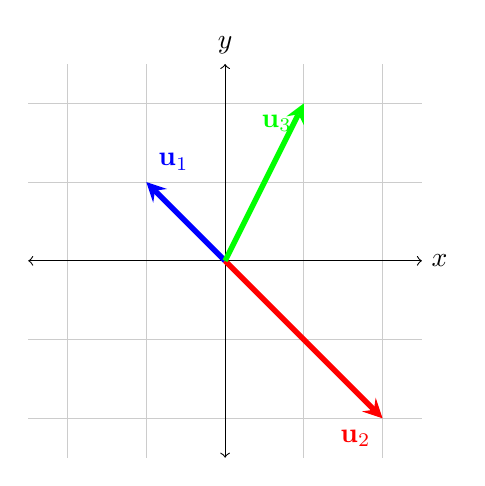
\begin{tikzpicture}
  \draw[thin,gray!40] (-2.5,-2.5) grid (2.5,2.5);
  \draw[<->] (-2.5,0)--(2.5,0) node[right]{$x$};
  \draw[<->] (0,-2.5)--(0,2.5) node[above]{$y$};
  \draw[line width=2pt,blue,-stealth](0,0)--(-1,1) node[anchor=south west]{$\boldsymbol{\mathbf{u}_1}$};
  \draw[line width=2pt,red,-stealth](0,0)--(2,-2) node[anchor=north east]{$\boldsymbol{\mathbf{u}_2}$};
  \draw[line width=2pt,green,-stealth](0,0)--(1,2) node[anchor=north east]{$\boldsymbol{\mathbf{u}_3}$};
\end{tikzpicture}
%
\caption{Grafisk illustration af mængderne $\S_1 \subset \S_2$.}
\label{span_eks}
\end{figure}
%
\end{eks}
%
%%%%%%%%%%%%%%%%%%%%%%%%%%%%%%%%%%%%%%%%%%%%%%%%%%%%%%%%%%%%%%%%%%%%%%%%
%
Typisk bruges span til at undersøge, hvorvidt en given vektor er i spannet for en vektormængde. 
Dette gøres ved at undersøge om en vektor kan konstrueres som linearkombination af vektorerne i mængden, hvilket undersøges ved hjælp af rækkereduktionsalgoritmen. 
\\
%
%%%%%%%%%%%%%%%%%%%%%%%%%%%%%%%%%%%%%%%%%%%%%%%%%%%%%%%%%%%%%%%%%%%%%%%%
%
\begin{eks}
%
Det skal undersøges, hvorvidt vektor $\mathbf{u}$ er i spannet for $\S_1$. 
Givet
\begin{align*}
\mathbf{v}= \begin{bmatrix}
           -1 \\
           2 \\
           3 \\
\end{bmatrix} 
\text{      }
\text{span}\{\S \} =
\left\{ 
\begin{bmatrix}
           1 \\
           2 \\
           1 \\
\end{bmatrix} 
,
\begin{bmatrix}
           1 \\
           1 \\
           0 \\
\end{bmatrix}
,
\begin{bmatrix}
           1 \\
           -1 \\
           -2 \\
\end{bmatrix}
\right\}.
\end{align*}
%
Dette opskrives nu som total-matricen
%
\begin{align*}
A=&
\begin{blockarray}{ccccc}
\mathbf{u}_1 & \mathbf{u}_2 & \mathbf{u}_3 & \mathbf{v} \\
\begin{block}{[ccc|c]c}
  1 & 1 & 1 & -1 \\
  2 & 1 & -1 & 2 \\
  1 & 0 & -2 & 3 \\
\end{block}
\end{blockarray} 
\end{align*}
%
Denne omskrives nu til trappeform
%
\begin{align*}
\xrightarrow[R_3 \rightarrow R_3-R_1]{R_2 \rightarrow R_2-2R_1}&
\begin{blockarray}{ccccc}
\mathbf{u}_1 & \mathbf{u}_2 & \mathbf{u}_3 & \mathbf{v} \\
\begin{block}{[ccc|c]c}
  1 & 1 & 1 & -1 \\
  0 & -1 & -3 & 4 \\
  0 & -1 & -3 & 4 \\
\end{block}
\end{blockarray} \\
%
\xrightarrow{R_3 \rightarrow R_3-R_2}&
\begin{blockarray}{ccccc}
\mathbf{u}_1 & \mathbf{u}_2 & \mathbf{u}_3 & \mathbf{v} \\
\begin{block}{[ccc|c]c}
  \hlight{1} & 1 & 1 & -1 \\
  0 & \hlight{-1} & -3 & 4 \\
  0 & 0 & 0 & 0 \\
\end{block}
\end{blockarray} 
\end{align*}
%
Ud fra dette ses det, at $\mathbf{v}$ er i $\text{span}\{\S \}$.
%
\end{eks}
%
%%%%%%%%%%%%%%%%%%%%%%%%%%%%%%%%%%%%%%%%%%%%%%%%%%%%%%%%%%%%%%%%%%%%%%%%
%
Egenskaberne vedrørende spannet kan udtrykkes på forskellige måder, hvilket leder til følgende sætning:
% 
\begin{thm}{}{spaneqv}
%
De følgende udsagn om en $m \times n$ matrix $A$ er ækvivalente:
%
\begin{enumerate}[label=(\alph*)]
\item Spannet af søjlerne i $A$ er $\R^m$.
\item Matricen $A\mathbf{x}=\mathbf{b}$ har mindst én løsning for alle $b$ i $\R^m$.
\item Rangen af $A$ er antallet af rækker $m$.
\item Den reducerede trappeform har ingen nulrækker.
\item Der er pivot-indgang i hver række i $A$. 
\end{enumerate}
%
\end{thm}
%
%
\begin{proof}
%
Udsagn (a) og (b) er ækvivalente, eftersom det er en forudsætning, at der kan skabes en linear kombination af $A\mathbf{x} =\mathbf{b}$ for ethvert $\mathbf{b}$ i $\R^m$, da det netop er definitionen af spannet, der dækker $\R^m$. 
%
Hvis der ikke er nogle nul-rækker i den reducerede trappeform, følger det, at $\text{rang}\{A\}$ er $m$, hvorfor (c) og (d) er ækvivalente. 
Eftersom matrixen er på reduceret trappeform, er denne derfor ækvivalent med (e).
\\\\
Det skal nu bevises at (b) og (c) er ækvivalente. 
Lad $B$ være den reducerede trappeform af $A$, og $\mathbf{e}_m$ er standard vektoren
%
\begin{align*}
\mathbf{\mathbf{e}_m} = \begin{bmatrix}
		0 \\
        \vdots \\
        0 \\
        1 
\end{bmatrix}
\end{align*}
%
i $\R^m$. 
Gennem rækkereduktionsalgoritmen kan $A$ transformeres til $B$. 
Da disse række er reversible, følger det, at der findes en sekvens af rækkeopperationer, som kan transformere $B$ til $A$.
Hvis disse opperationer udføres på totalmatricen 
$[B \text{    } \mathbf{e}_m]$ 
for at konstruere matricen 
$[A \text{    } \mathbf{d}]$, 
$\mathbf{d} \in \R^n$, 
så følger det, at ligningssystemet $A\mathbf{x}=\mathbf{
d}$ er ækvivalent med $B\mathbf{x}=\mathbf{e}_m$.
\\\\
Hvis (b) er sand, følger det, at de to ligningssystemer er konsistente. 
Det følger derfor af sætning \ref{thm:konsistens}, at den sidste række ikke kan være en nulrække, da standardvektoren $\mathbf{e}_m$ vil have pivotindgang i sidste søjle og derfor vil ligningssystemet være inkonsistent.
Dermed er $rang(A)=m$, hvilket leder til (c).
% Dette kan eventuelt forklares dybere xD
\\\\
Antag, at (c) er sand. 
Lad $[B \text{    }| \mathbf{c}]$ 
være den reducerede trappeform af 
$[A \text{    } | \mathbf{b}]$.
Eftersom $A$ har rangen $m$, følger det, at der ikke findes en nulrække i $B$.
Derfor kan $[B \text{    } \mathbf{c}]$ ikke indeholde en nulrække, hvis eneste nulindgang er i sidste søjle. 
Det følger derfor jævnfør sætning \ref{thm:konsistens}, at $A\mathbf{x}=\mathbf{b}$ er konsistent $\forall \mathbf{b}$, hvilket beviser at (b) og (c) er ækvivalente.
%
\end{proof}
\\
%
%%%%%%%%%%%%%%%%%%%%%%%%%%%%%%%%%%%%%%%%%%%%%%%%%%%%%%%%%%%%%%%%%%%%%%%%
%
Når det skal afgøres, hvorvidt en vektor tilhører et givet span, gælder sætning \ref{thm:span}.
%
\begin{thm}{}{span}
%
Lad $\S =  \{ \mathbf{u}_1, \mathbf{u}_2 , \ldots , \mathbf{u}_k \}$ være en mængde vektorer i $\R^n$, og lad $\mathbf{v}$ være en vektor i $\R^n$.
Så er $\text{span}\{ \mathbf{u}_1, \mathbf{u}_2 , \ldots , \mathbf{u}_k , \mathbf{v}\} =\text{span}\{\S\}$, hvis og kun, hvis $\mathbf{v}$ tilhører $\text{span}\{\S\}$.
%
\end{thm}
%
%
\begin{proof}
%
Antag, at $\mathbf{v}$ er i $\text{span}\{\S\}$. Så er $\mathbf{v}$ en linearkombination af $\S$, hvilket kan opskrives som $\mathbf{v}=a_1\mathbf{u}_1+a_2\mathbf{u}_2+ \ldots + a_k\mathbf{u}_k$, hvor $a_1,a_2,\ldots, a_k$ er skalarer. 
Hvis en vektor $\mathbf{w}$ er i $\text{span}\{ \mathbf{u}_1, \mathbf{u}_2 , \ldots , \mathbf{u}_k , \mathbf{v}\}$, 
kan denne opskrives $\mathbf{w}=c_1\mathbf{u}_1+c_2\mathbf{u}_2+ \ldots + c_k\mathbf{u}_k+b\mathbf{v}$, hvor $c_1,c_2,\ldots, c_k, b$ er skalarer.
Ved substitution af $\mathbf{v}$ med $\{ \mathbf{u}_1, \mathbf{u}_2 , \ldots , \mathbf{u}_k , \mathbf{v}\}$ vides det, at $\mathbf{w}$ kan opskrives som en linearkombination af $\S$. 
Det gælder endvidere, at alle linearkombinationer i $\S$ også kan dannes fra vektorerne $\mathbf{u}_1,\mathbf{u}_1, \mathbf{u}_2 , \ldots , \mathbf{u}_k , \mathbf{v}$, hvis $\mathbf{v}$ multipliceres med skalaren $0$.
Det følger derfor, at de to mængder har samme span. 
Antag nu, at $v$ ikke er i $\text{span}\{\S\}$. 
Det følger herfra, at $\mathbf{v}$ er i spannet af 
$\{ \mathbf{u}_1,\mathbf{u}_1, \mathbf{u}_2 , \ldots , \mathbf{u}_k , \mathbf{v}\}$, da 
$\mathbf{v}=0\mathbf{u}_1+0\mathbf{u}_2+ \ldots + 0\mathbf{u}_k+1\mathbf{v}$.
Derfor er
$\text{span}\{ \mathbf{u}_1,, \mathbf{u}_2 , \ldots , \mathbf{u}_k \}
\neq
\text{span}\{ \mathbf{u}_1,, \mathbf{u}_2 , \ldots , \mathbf{u}_k , \mathbf{v}\}$, 
da mængderne ikke er ækvivalente, idet kun én af dem indeholder $\mathbf{v}$. 
%
\end{proof}
\\
%
%%%%%%%%%%%%%%%%%%%%%%%%%%%%%%%%%%%%%%%%%%%%%%%%%%%%%%%%%%%%%%%%%%%%%%%%
%
Som det fremgår af overstående gælder det derfor, at enhver løsning i et lineært optimeringsproblem skal findes i spannet for vektorerne i ligningssystemet. 
%
	
% LINEÆR OPTIMERINGSPROBLEMER 
	% Generel definition - Optimering 
	\chapter{Lineær optimeringsproblemer}
% God arbejdslyst 
	% Standartform 
	\section{Standardform}
\label{sec:standard}
% 
Hvis et lineært optimeringsproblem er på formen
%
\begin{align*}
\begin{array}{lrl}
\text{Maksimér}		&\textbf{c}^T\textbf{x}	&				\\
\text{begrænset af}	&A\textbf{x}	&=\mathbf{b},	\\
					&\mathbf{x}				&\geq \mathbf{0},
\end{array}
\end{align*}
%
er optimeringsproblemet på \textit{standardform}.
Bemærk, at problemet på standardform er et maksimumsproblem, og betingelserne er lighedsbetingelser og ikke-negativsbetingelser.
\\\\
%
For at omskrive et minimumsproblem til et maksimumsproblem multipliceres objektfunktionen med $-1$.
Ulighedsbetingelserne ændres ligeledes fra $A_ix_i \geq b_i$ til $-A_ix_i \leq -b_i$.
\\\\
%
For at få et givet problem med ulighedsbetingelser på standardform tilføjes \textit{slack-variable} til venstre side af ulighederne for at gøre dem til ligheder. 
Hvis optimeringsproblemet har $m$ uligheder tilføjes $m$ slack-variabler.
I denne rapport noteres slack-variabler $s_i$.
Variabler, der ikke har en ikke-negativsbegrænsning, opdeles i $x_i^+$ og $x_i^-$, da alle reelle tal kan skrives som differensen mellem to positive tal.
Dertil isoleres objektfunktionen så $z$ er positiv på ventre side af lighedstegnet og sættes lig nul.
Med denne fremgangsmåde kan alle lineære optimeringsproblemer omskrives til standardform.
Det er derfor kun nødvendigt med en metode til at løse optimeringsproblemer på denne form.
%
%\begin{align*}
%\sum^n_{i=1} \mathbf{A}_i x_i = \mathbf{b}.
%\end{align*}

%\begin{align*}
%\begin{array}{lrl}
%\text{Minimer}		&\textbf{c}^T\textbf{x}	&				\\
%\text{begrænset af}	&\textbf{A}\textbf{x}	&=\mathbf{b},	\\
%					&\mathbf{x}				&\geq \mathbf{0},		
%\end{array}
%\end{align*}
%
\begin{eks}
Minimumsproblemet fra eksempel \ref{eks:min_lin} er her omskrevet til standardform:
%
\begin{align*}
\begin{array}{lrcccrcrcrcrcrcr}
\text{Maksimér}		&	\multicolumn{2}{c}{-4x_1 + 3x_2}\\
\text{begrænset af}	&2x_1	&-	&x_2^+-x_2^-		&+	&s_1&	&	&	&	&	&	&= 		&-10,\\
					&-x_1	&+	&x_2^+-x_2^-		&	&	&+	&s_2&	&	&	&	&=		& -7,\\
					&x_1	&+	&x_2^+-x_2^-		&	&	&	&	&+	&s_3&	&	&=		& 20,\\
					& 		&	&x_2^+-x_2^-&	&	&	&	&	&	&+	&s_4&=		& 12,\\
					&x_1	&	&			&	&	&	&	&	&	&	&	&\geq	& 0,\\
					&		&	&x_2^+,x_2^-&	&	&	&	&	&	&	&	&\geq	& 0.\\
\end{array}
\end{align*}
\end{eks}
%
	% Slack varialbe 
	\section{Slack variable}
% God arbejdslyst 
	% Dualitet 
	\newpage
\section{Dualitet}
% Vi kan vælge at tage det med lagrange multiplier med også men tænker vi snakker om det jeg er personligt i tvivl og ville nødigt spilde tiden på det.
	% - Julie: Jeg synes ikke vi skal have det med 
% Jeg er iøvrigt bange for jeg er kommet til at skyde mig selv i foden, men umiddelbart giver det mening for mig, det snakker vi om.
	% - Julie: Jeg tror du har styr på det xD
%
Et vigtigt element af teorien vedrørende lineære optimeringsproblemer og simplexmetodens brug omhandler \textit{dualproblemer}.
%
\begin{defn}{}{dualproblemer}
Givet maksimumsproblemet
%
\begin{align*}
\begin{array}{lrll}
\text{Maksimér}		&\textbf{c}^T\textbf{x}	&=z			&\\
\text{begrænset af}	&\textbf{a}_i^T\textbf{x}	&\geq b_i,	&i \in M_1,\\
					&\textbf{a}_i^T\textbf{x}	&\leq b_i,	&i \in M_2,\\
					&\textbf{a}_i^T\textbf{x}	& = b_i,	&i \in M_3,\\
					&x_j					&\geq 0,	&j \in N_1,\\
					&x_j					&\leq 0,	&j \in N_2,\\							&x_j					&\text{fri},	&j \in N_3.
\end{array}
\end{align*}
%
Da vil \textbf{dual minimumsproblemet} være
% Minimer $v=\mathbf{b}^T \mathbf{p}$ begrænset af $A^T \mathbf{p} \geq c$ og $\mathbf{p} \geq 0$
%
\begin{align*}
\begin{array}{lrll}
\text{Minimér}		&\textbf{p}^T\textbf{b}	&=v			&\\
\text{begrænset af}	&p_i					&\geq 0,	&i \in M_1,\\
					&p_i					&\leq 0,	&i \in M_2,\\
					&p_i					&\text{fri},	&i \in M_3,\\
					&\textbf{p}^T\textbf{A}_j	&\leq c_j,	&j \in N_1,\\
					&\textbf{p}^T\textbf{A}_j	&\geq c_j,	&j \in N_2,\\
					&\textbf{p}^T\textbf{A}_j	& = c_j,	&j \in N_3.
\end{array}
\end{align*}
%
\end{defn}
\noindent
%
Problemet
%
\begin{align*}
\begin{array}{lrl}
\text{Maksimér}		&\textbf{c}^T\textbf{x}	& = z		\\
\text{begrænset af}	&A\textbf{x}	&\leq \mathbf{b},	\\
					&\mathbf{x}				&\geq \mathbf{0},
\end{array}
\end{align*}
%
vil således have
%
\begin{align*}
\begin{array}{lrl}
\text{Minimér}		&\textbf{p}^T\textbf{b}	& = v			\\
\text{begrænset af}	&\textbf{p}^TA	&\leq \mathbf{c},	\\
					&\mathbf{b}				&\leq \mathbf{0}
\end{array}
\end{align*}
%
som dualproblem.
%Ideer til en federe opsætning
\\\\
%
For hver begrænsning i det oprindelige problem indføres således en variabel i dualproblemet.
Tilsvarende indføres en begrænsning for hver variabel. 
Derudover skiftes fra et maksimums- til minimumsproblem.
I tabel \ref{juliedum} ses en oversigt over egenskaber ved primærproblemet og dettes dualproblem.\\
%
\begin{table}[H]
\begin{center}
\begin{tabular}{llll}
Primær  & Maksimér   & Minimér    & Dual         \\
\hline
Begræsninger & $\leq b_i$ & $\geq 0$   & Variable     \\
             & $\geq b_i$ & $\leq 0$   &              \\
             & $=b_i$     & fri        &            \\ 
\hline             
Variable     & $\geq 0$   & $\geq c_j$ & Begræsninger \\
             & $\leq 0$   & $\leq c_j$ &              \\
             & fri        & $=c_j$     &  
\end{tabular}
\end{center}
\captionof{table}{Oversigt over egenskaber ved primærproblemet og dettes dual.}
\label{juliedum}
%\captionof{tabular}{Fisk finder i på noget.}
\end{table}
\noindent
%
Dualproblemet kan således opstilles som i \ref{dual}. \\
%
\begin{eks}
\label{dual}
%
Betragt primærproblemet
%
\begin{align*}
\begin{array}{lrrlr}
\text{Maksimér}		&	\multicolumn{2}{c}{5x_1+4x_2}  & = & z\\
\text{begrænset af}	&3x_1& +5x_2			&\leq 	&78,\\
					&4x_1& + x_2				&\leq	& 36,\\
					&x_1,&  x_2				&\geq	& 0.
\end{array}
\end{align*}
\\
Dualproblemet vil således have formen
%hvilket bogstave foretrækker i istedet for z? hvis i vil ha z i standard notationen 
	% Julie: Tænker v? var det ikke det du skrev i den forrige?
\begin{align*}
\begin{array}{lrrlr}
\text{Minimér}		&	\multicolumn{2}{c}{78p_1+36p_2}  & =  & v\\
\text{begrænset af}	&3p_1& +4p_2			&\geq 	&5,\\
					&5p_1& + p_2				&\geq	& 4,\\
					&p_1,&  p_2				&\geq	& 0.
\end{array}
\end{align*}
% 
%I afsnit \ref{coronaaaaaaaaaaa} vil dette eksempel blive belyst. Dualproblemet vil istedet minimere indholdet af sukker og kulhydrater begrænset af forholdet mellem to typer slik i en slikpose.
%
\end{eks}
%
%Som det fremgår i eksemplet har løsningen på dualproblemet samme optimale løsning, hvor slackvariable her er løsningen på det oprindelige problem.
%
Det gælder endvidere, at der fra dualproblemet kan vendes tilbage til det oprindelige problem, hvilket udtrykkes ved \ref{thm:dualitetsaet}.
%
\begin{thm}{}{dualitetsaet}
Hvis dualproblemet omdannes til et ækvivalent minimumsproblem og dualproblemet af minimumsproblemet dannes, opnås primærproblemet.
\end{thm}
%
\newpage
%
\begin{proof}
Betragt problemet
\begin{align*}
\begin{array}{lrll}
\text{Minimér}		&\textbf{p}^T\textbf{b}		&= z		&\\
\text{begrænset af}	&p_i						&\geq 0,	&i \in M_1,\\
					&p_i						&\leq 0,	&i \in M_2,\\
					&p_i						&\text{fri},&i \in M_3,\\
					&\textbf{p}^T\textbf{A}_j	&\leq c_j,	&j \in N_1,\\
					&\textbf{p}^T\textbf{A}_j	&\geq c_j,	&j \in N_2,\\
					&\textbf{p}^T\textbf{A}_j	& = c_j,	&j \in N_3,
\end{array}
\end{align*}
og dets dualproblem
\begin{align*}
\begin{array}{lrll}
\text{Maksimér}		&\textbf{c}^T\textbf{x}		&= v		&\\
\text{begrænset af}	&\textbf{a}_i^T\textbf{x}	&\geq b_i,	&i \in M_1,\\
					&\textbf{a}_i^T\textbf{x}	&\leq b_i,	&i \in M_2,\\
					&\textbf{a}_i^T\textbf{x}	& = b_i,	&i \in M_3,\\
					&x_j						&\geq 0,	&j \in N_1,\\
					&x_j						&\leq 0,	&j \in N_2,\\
					&x_j						&\text{fri},&j \in N_3.
\end{array}
\end{align*}
Dualproblemet omdannes til det ækvivalente minimumsproblem
\begin{align*}
\begin{array}{lrll}
\text{Minimér}		&-\textbf{c}^T\textbf{x}	&=-v		&\\
\text{begrænset af}	&-\textbf{a}_i^T\textbf{x}	&\leq -b_i,	&i \in M_1,\\
					&-\textbf{a}_i^T\textbf{x}	&\geq -b_i,	&i \in M_2,\\
					&-\textbf{a}_i^T\textbf{x}	& = -b_i,	&i \in M_3,\\
					&x_j						&\geq 0,	&j \in N_1,\\
					&x_j						&\leq 0,	&j \in N_2,\\
					&x_j						&\text{fri},&j \in N_3.
\end{array}
\end{align*}
Dualproblemet til dette er
\begin{align*}
\begin{array}{lrll}
\text{Maksimér}		&-\textbf{p}^T\textbf{b}	&=-z		&\\
\text{begrænset af}	&p_i					&\geq 0,	&i \in M_1,\\
					&p_i					&\leq 0,	&i \in M_2,\\
					&p_i					&\text{fri},	&i \in M_3,\\
					&-\textbf{p}^T\textbf{A}_j	&\geq -c_j,	&j \in N_1,\\
					&-\textbf{p}^T\textbf{A}_j	&\leq -c_j,	&j \in N_2,\\
					&-\textbf{p}^T\textbf{A}_j	& = -c_j,	&j \in N_3,
\end{array}
\end{align*}
%
hvilket har det ækvivalente minimumsproblem
%
\begin{align*}
\begin{array}{lrll}
\text{Minimér}		&\textbf{p}^T\textbf{b}	&=z			&\\
\text{begrænset af}	&p_i					&\geq 0,	&i \in M_1,\\
					&p_i					&\leq 0,	&i \in M_2,\\
					&p_i					&\text{fri},	&i \in M_3,\\
					&\textbf{p}^T\textbf{A}_j	&\leq c_j,	&j \in N_1,\\
					&\textbf{p}^T\textbf{A}_j	&\geq c_j,	&j \in N_2,\\
					&\textbf{p}^T\textbf{A}_j	& = c_j,	&j \in N_3,
\end{array}
\end{align*}
%
som er identisk med primærproblemet. 
%
\end{proof}
%
%42 min https://youtu.be/0TRxEvMRE7s definition
	
% GEOMETRISK FREMSTILLING 
	\chapter{Grafisk løsning}
% 2.1 Polyeder og konvekse mængder 
% ---------------------------------------------------------
	\input{incl/main/grafisk_losning/hyperplan_halvrum_polyeder}
	\input{incl/main/grafisk_losning/konvekse_maengder}
% 
% 2.2 Ekstrema, hjørnepunkter og basale mulige løsninger 
% ---------------------------------------------------------
	\begin{defn}{}{algh}
Hvis en vektor $\textbf{x}$ opfylder $\textbf{a}^T_i\textbf{x}= b_i$ for $i \in M_1, M_2 \text{ eller } M_3$, så siges den tilsvarende betingelse at være \textbf{bindende} ved $\textbf{x}$.
\end{defn}\noindent
%
Følgende sætning giver anledning til hvordan disse bindende betingelser kan føres i relation til løsninger af lineære optimeringsproblemer.
%
\begin{thm}{}{}

Lad $\textbf{x}$ være et element i $\R^n$ og lad $I=\{i|\textbf{a}^T_i\textbf{x}=b_i\}$ være en mængde af indexer på betingelser, der er bindende ved $\textbf{x}$.
Så er følgende udsagn ækvivalente.
%
\begin{enumerate}[label=(\alph*)]
\item Der eksisterer $n$ vektorer i mængden $\{\textbf{a}_i|i \in I \}$, som er lineært uafhængige.
\item Spannet af vektorerne $\textbf{a}_i$, for $i$ i $I$, dækker hele $\R^n$.
\item Ligningssystemet $\textbf{a}^T_i\textbf{x}= b_i$, for $i \in I$, har en entydig løsning.
\end{enumerate}
\end{thm}
%
\begin{proof}
Smukt bevis INC.
\end{proof}
	\section{Ekstremer, hjørnepunkter og basale løsninger}
%
%\textit{Vis at løsningerne findes i hjørnene af en polytede.}
Som det fremgår af afsnit \ref{heeeeejjulle}, vil en optimal løsning være tilbøjelige til at ligge i hjørnerne af en polyede.
Der er derfor behov for måder at definere disse hjørner på.
%
\begin{defn}{}{ekstrema}
Lad $\mathcal{P}$ være en polyede. 
En vektor $\mathbf{x} \in \mathcal{P}$ kaldes et \textbf{ekstremumspunkt} i $\mathcal{P}$, hvis der ikke eksisterer to vektorer $\mathbf{y},\mathbf{z} \in \mathcal{P}$, $\mathbf{y} \land \mathbf{z} \neq \mathbf{x}$, 
samt en skalar $\lambda \in [0,1]$, hvorom det gælder: $\mathbf{x}=\lambda\mathbf{y}+(1-\lambda)\textbf{z}$.
\end{defn}
\noindent
%
%
Et hjørne kan beskrives ud fra denne definition idet der såfremt $\mathbf{x}=\lambda\mathbf{y}+(1-\lambda)z$, og alle vektorene findes i $P$, gælder at $\mathbf{x}$ er en konveks kombination af $\mathbf{y}$ og $\mathbf{z}$.
Hvis $\mathbf{x}=\lambda\mathbf{y}+(1-\lambda)\textbf{z}$ og $\mathbf{x}$ er et ekstremumspunkt må det derfor gælde at $\mathbf{y}\notin P$ eller $\mathbf{z}\notin P$ eller $\mathbf{x}=\mathbf{z}$ eller $\mathbf{x}=\mathbf{y}$. 
Det skal her nævnes at denne definition er strengt geometrisk.
%

\begin{figure}[h!]
  \centering
  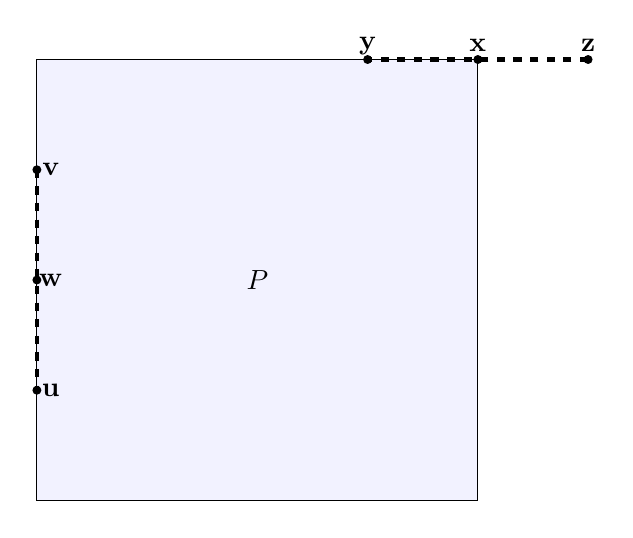
\begin{tikzpicture}[scale=0.7]
    \tikzset{punkt/.style={point, draw=black}}
    
    
%Punkter

	\node at (4,4)	(1){};
	\node at (-4,4)	(4){};
	\node at (4,-4)	(2){};
	\node at (-4,-4) (3){};


	\filldraw[black, fill=blue!5] (2) rectangle (4);
	\node at (0,0) (P){$P$};
	
	\filldraw [black] (2,4) circle (2pt);
	\filldraw [black] (4,4) circle (2pt);
	\filldraw [black] (6,4) circle (2pt);
	\filldraw [black] (-4,2) circle (2pt);
	\filldraw [black] (-4,0) circle (2pt);
	\filldraw [black] (-4,-2) circle (2pt);	
	\node at (2,4.25)	 (y){$\textbf{y}$};
	\node at (4,4.25)	 (x){$\textbf{x}$};
	\node at (6,4.25)	 (z){$\textbf{z}$};
	\node at (-3.75,2)  (v){$\textbf{v}$};
	\node at (-3.75,0)	 (w){$\textbf{w}$};
	\node at (-3.75,-2) (u){$\textbf{u}$};


	\draw[-, dashed,black,ultra thick] (6,4) -- (2,4);
	\draw[-, dashed,black,ultra thick] (-4,2) -- (-4,-2);

  \end{tikzpicture}
  \caption{En afgrænset polytop $P$ hvor $\textbf{x}$ er et ekstramapunkt da der ikke findes vektorer $\textbf{y}$ og $\textbf{z}$ sådan at $\mathbf{x}=\lambda\mathbf{y}+(1-\lambda)z$. $\textbf{w}$ er i modsætning ikke et ekstremapunkt da der findes $\textbf{v}$ og $\textbf{u}$ sådan at $\mathbf{w}=\lambda\mathbf{v}+(1-\lambda)u$.}
  \label{fig:ekstrema}
\end{figure}
%
%
%    \node[punkt] at (-4,0.5)      (v1){$v_1$};
%    \node[punkt] at (-2,0.5)      (v2){$v_2$};
%    \node[punkt] at (-4,-1.5)     (v3){$v_3$};
%    \node[punkt] at (-2,-1.5)     (v4){$v_4$};
%    \node at (-3,2)     (v){$K_{4}$};
%
%
%    \node[punkt] at (4.6,-0.2)      (k1){$v_3$};
%    \node[punkt] at (1.4,-0.2)      (k2){$v_2$};
%    \node[punkt] at (2,-2)     (k3){$v_4$};
%    \node[punkt] at (4,-2)     (k4){$v_5$};
%    \node[punkt] at (3,1)      (k5){$v_1$};
%    \node at (3,2)      (k){$K_{5}$};
%
%
%
%
%
%    \draw [-, thick, draw=black] (v1) -- (v2);
%    \draw [-, thick, draw=black] (v1) -- (v3);
%    \draw [-, thick, draw=black] (v1) -- (v4);
%    \draw [-, thick, draw=black] (v2) -- (v3);
%    \draw [-, thick, draw=black] (v2) -- (v4);
%    \draw [-, thick, draw=black] (v3) -- (v4);
\\\\
%
En alternativ geometrisk definition relatere sig til \textit{hjørne punkter}, som er den entydige optimale løsning til et givet lineært programmeringsproblem med den mulige løsningsmængde $\mathcal{P}$.
%
\begin{defn}{}{hjoerner}
Lad $P$ være en polyede. 
En vektor $\mathbf{x}\in P$ siges at være et \textbf{hjørne punkt}, hvis der esksiterer en vektor $\mathbf{c}$, hvorom det gælder at $\mathbf{c}^T\mathbf{x}<\mathbf{c}^T\mathbf{y}$ for alle $\mathbf{y}$, som opfylder $\mathbf{y} \in P$ samt $\mathbf{y}\neq\mathbf{x}$.
\end{defn}
\noindent
%
%
Dette kan ligeledes beskrives som at $\mathbf{x}$ er et hjørne i $P$ såfremt $P$ er på den ene side af et hyperplan der skærer $P$ i $\mathbf{x}$. 
Jævnfør definitionen har dette hyperplan ligningen $y \mid \mathbf{c}^T\mathbf{x}=\mathbf{c}^T\mathbf{y}.$
% 
% 2.3 Polyede på standardform
% ---------------------------------------------------------
	\section{Polyeder på standardform}
\label{afsnit:fisk}
%
Som det bliver beskrevet i afsnit \ref{sec:standard} kan optimeringsproblemer opskrives på standardform.
Dette korosponderer med polyeder der ligeledes kan opskrives på standardform: 
$P=\{ \mathbf{x} \in \R^n \mid A\mathbf{x}=\mathbf{b},x \geq 0 \}$, hvor er $A$ er en $m \times n$ matrix.
$P$ bliver er her et \textbf{polyede på standardform}.
I de fleste tilfælde er det en fordel at antage at de $m$ rækker i $A$ er lineært uafhængige.
%I sætning \ref{something something} vil det endvidere blive vist at rækker der ikke er uafhængige kan udelukkes fra løsningen.
som det ses i (ref til basale mulige løsninger) skal der være $n$ aktive-begrænsninger i spil for at finde en basal mulig løsning.
såfremt $m \neq n$, skal der derfor vælges $n-m$ variable $x_i$ med henblik på, at sætte disse $x_i=0$, hvilket gør begrænsningerne $x_i \geq 0$ aktive.
ovenstående 53 i bogen har behov for andre læser så vi kan diskutere hvad det betyder.
Det er dog ikke uvæsentligt hvilke af disse variable der omdannes til $0$ hvilket belyses af sætning \ref{thm:polystd}.
\begin{thm}{}{polystd}
Ved begrænsningerne $A\mathbf{x}=\mathbf{b}$ og $\mathbf{x}\geq 0$.
Antag at $A$ er en $m \times n$ og har lineært uafhængige rækker.
$\mathbf{x} \in \R^n$ er en basal løsning hvis og kun hvis: $A\mathbf{x}=\mathbf{b}$ og der eksisterer indexer $B(1),\ldots,B(m)$ hvorom det gælder:
\begin{enumerate}[label=(\alph*)]
\item Søjlerne $\mathbf{A}_{B(1)},\ldots,\mathbf{A}_{B(m)}$ er lineært uafhængige.
\item Hvis $i \neq \mathbf{A}_{B(1)},\ldots,\mathbf{A}_{B(m)}$, så er $x_i=0$.
\end{enumerate}
\end{thm}
\begin{proof}
Betragt et $x \in \R^n$ og antag at der eksiterer indexer $\mathbf{A}_{B(1)},\ldots,\mathbf{A}_{B(m)}$ der opfylder (a) og (b).
Da gælder om de aktive begrænsninger at $x_i=0$, når $i\neq B(1),\ldots,B(m)$, samt at $A\mathbf{x}=\mathbf{b}$.
Dette implicere, da liniært afhængige løsninger sættes lig $0$,  at 
$$\sum_{i=1}^{m}\textbf{A}_{B(i)}x_{B(i)}=\sum_{i=1}^{n}\textbf{A}_ix_i=A\textbf{x}=\textbf{b}$$.
Da søjlerne $\textbf{A}_{B(i)}x_{B(i)}$ for $i=1,\ldots,m$ er lineært uafhængige, kan $x_{B(1)},\ldots,x_{B(m)}$ bestemmes entydigt. 
Altså har ligningssystemet skabt af de aktive begrænsninger en entydig løsning.
Fra sætning (MAAADS), følger at der er $n$ aktive begrænsninger, hvorfor $\mathbf{x}$ er en basal løsning. 
Antag nu at $\mathbf{x}$ er en basal løsning, det skal nu vises at (a) og (b) da er opfyldt.
Lad $x_{B_1},\ldots,x_{B_k}$ være ikke-nul komponenter i $\textbf{x}$.
Da $\mathbf{x}$ er en basal løsning, følger nu at ligningssysemet givet ved de aktive begrænsninger $x_i=0$, når $i\neq B(1),\ldots,B(k)$, samt  $\sum_{i=1}^{n}\mathbf{A}_ix_i=\mathbf{b}$, har en entydig løsning. 
Det samme må derfor gøre sig gældende for $\sum_{i=1}^{k}\mathbf{A}_{B(i)}x_{B(i)}=\mathbf{b}$.
Det følger derfor at søjlerne i $A_{B(1)},\ldots,A_{B(k)}$ er lineært uafhængige.
Hvis dette ikke var tilfældet ville der findes løsninger til $\sum_{i=1}^{k}\mathbf{A}_{B(i)} x_{B(i)}=\mathbf{0}$ udover den trivielle, hvilket betyder løsningen $\mathbf{x}$ ikke er entydig, dette er i modstrid til at denne er en basal løsning.
$\mathbf{A}_{B(1)},\ldots ,\mathbf{A}_{B(k)}$ er således lineært uafhængige og $k \leq m$.
Da $A$ har $m$ lineært uafhængige rækker, er der ligeledes $m$ lineært uafhængige søjler.
%her kommer noget der følger fra sætning 1.3 i sektion 1.5 tror ikke vi har noget tilsvarende.
Der kan derfor findes $m-k$ søjler $A_{B(k+1)},\ldots,A_{B(m)}$ hvorom det gælder at søjlerne $\mathbf{A}_{B(i)}$ med $i=1,\ldots,m$, er lineært uafhængige.
Da $k \leq m$ gælder det hvis $i \neq B(1),\ldots,B(m)$ at $i \neq B(1),\ldots,B(k)$ og $x_i=0$.
\end{proof}
%der skal flere igennem det her bevis, tænker det er svært for andre end mig.	

% SIMPLEX METODEN
	\chapter{Simplex metoden}
% God arbejdslyst 	

% LU - DEKOMPOSITION 
	\chapter{LU-dekomposition}
% God arbejdslyst 

% Appendicer indsættes inde i en appendices-blok og bliver nummereret med
% bogstaver i stedet for tal
\begin{appendices}

\end{appendices}

% Dokumentets 'back matter' er til ekstra ting som f.eks. litteraturlisten.
% Overskrifter bliver ikke nummereret her.
\backmatter

% Automatisk litteraturliste baseret på, hvilke kilder, der er blevet refereret
% til i løbet af rapporten.
\bibliographystyle{apalike}
\bibliography{
  incl/bib/books,
  incl/bib/articles,
  incl/bib/software
}

\end{document}
